\section{Randomized Algorithms}
When designing an algorithm, introducing the concept of randomization allows for simplest, fastest, or only known algorithm for a particular problem.In practise it relies heavily on a random number generator (we must assure that the number generator used is truly random).

\subsection{Contention Resolution}

Given n processes (that can't comunicate between themself) $P_{1}, ..., P_{n}$, each competing for access to a shared database: if two or more processes access the database simultaneously, all processes are locked out.\\ Devise protocol to ensure all processes get through on a regular basis.\\\\
For this particular problem does not exist a deterministic algorithm so we can either give to each process a timeslot at random or access/cannot access, note that every process must access in a finite amount of time.

\begin{figure}[H]
    \centering
    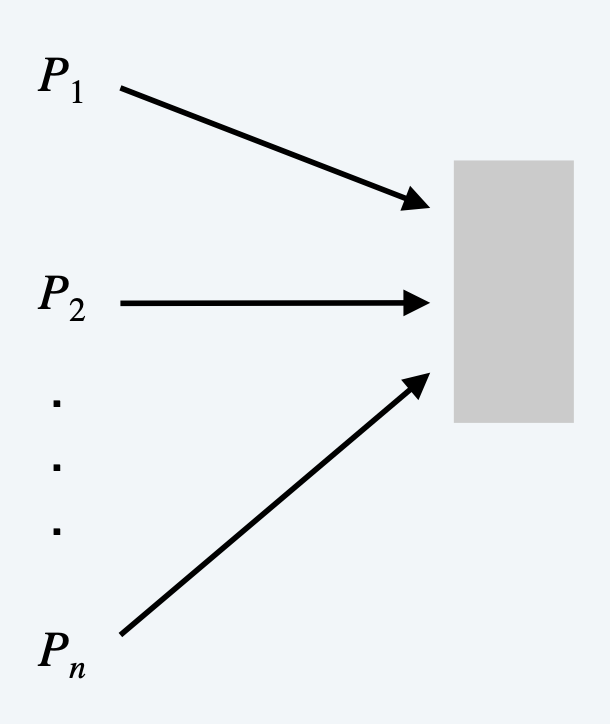
\includegraphics[width=0.2\textwidth ]{processes}
    \caption{Instance of the Content Resolution Problem}
\end{figure}

Each problem access with probability $p=\frac{1}{n}$, this is the value that maximize the event $Pr[S(i, t)]$ (probability that process i access the resource).Again let $S[i, t]$ = event that process i succeeds in accessing the database at time t,then:

\[ \frac{1}{(e⋅n)} \leq Pr [S(i, t)] \leq \frac{1}{2n} \]

with \emph{e} number of nepero, by independence we have:

\[Pr [S(i, t)] = p(1 – p)^ {n – 1}.\]

With p current process and 1-p all the other processes that attempts to access the resource, finally setting p = 1/n (value that maximize the event), we have:

\[Pr [S(i, t)] = \frac{1}{n}(1 – \frac{1}{n})^ {n – 1}.\]

This value is between $\frac{1}{e}$ and $\frac{1}{2}$.\\

\begin{claim}
    The probability that process i fails to access the database in en rounds is at most $\frac{1}{e}$. After $en (c ln n)$ rounds, the probability $\leq n^{-c}$.
\end{claim}\\

\begin{proof}
    Let F[i, t] = event that process i fails to access database in rounds 1 through t. By independence and previous claim, we have $Pr [F[i, t]] \leq (1 – \frac{1}{en}) t$.
\end{proof}\\

\begin{claim}
    The probability that all processes succeed within 2e ⋅ n ln n rounds is $\geq 1 – \frac{1}{n}$.
\end{claim}\\

\begin{proof}
    Let F[t] = event that at least one of the n processes fails to access database in any of the rounds 1 through t:

    \[Pr[F[t]]=Pr[ \cup_{i=1} F[i,t]] \leq \sum_{i=1}^{n} Pr[F[i,t]] \leq n(1−\frac{1}{en})^{t}\]

    The above equality is obtained by using the \emph{Union Bound}:
    \[Given \; the \; events \; E_{1}, ..., E_{n}, Pr[\cup_{i=1}^{n}E_{i}] \leq \sum_{i=1}^{n}Pr[E_{i}]\]

\end{proof}

\subsection{Global Minimum Cut}
Given a connected, undirected graph G=(V,E) find a cut (A, B) of minimum cardinality.\\

\emph{The contraction algorithm}:\\
Pick an edge e=(u,v) at random, then contract it:

\begin{itemize}

    \item {replace u and v by single new super-node w}\\
    \item {preserve edges, updating endpoints of u and v to w}\\
    \item{keep parallel edges, but delete self-loop}\\

\end{itemize}

Repeat until graph has just two nodes u1 and v1 and return the cut.

\begin{figure}[H]
    \centering
    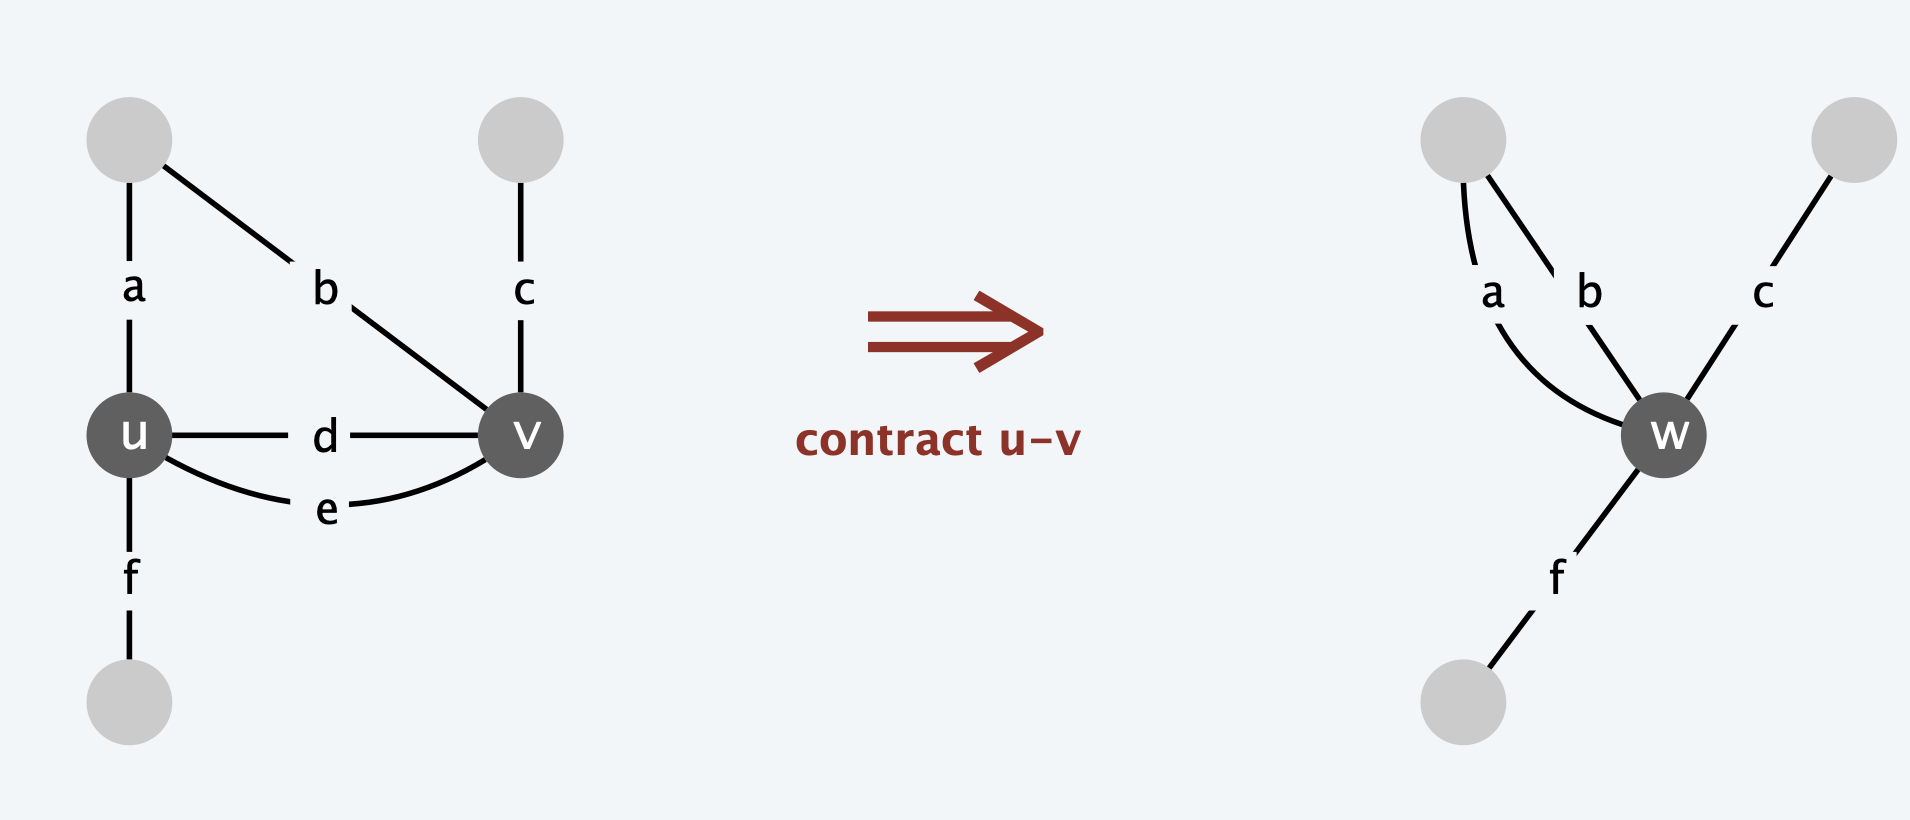
\includegraphics[width=0.6\textwidth ]{contract}
    \caption{The contract operation on G=(V,E)}
\end{figure}

\begin{claim}
    The contraction algorithm returns a min cut with prob $\geq \frac{2}{n^{2}}$ in $\mathcal{O}(m log3 n)$ .
\end{claim}\\

\begin{proof}
    Consider a global min-cut (A*, B*) of G: Let F* be edges with one endpoint in A* and the other in B* with k = $| F^{*} |$ = size of min cut.\\
    In first step, algorithm contracts an edge in F* probability $\frac{k}{| E |}$. Every node has degree $\geq$ k since otherwise (A*, B*) would not be a min-cut $\Rightarrow$ $| E | \geq \frac{1}{2} k n ⇔ \frac{k}{| E |} \leq 2 / n$, thus, algorithm contracts an edge in F* with probability $\leq \frac{2}{n}$.
\end{proof}\\

To amplify the probability of success run the contraction algorithm many times (for a formal proof please check professor's slides).

\subsection{Linearity of Expectation}

Expectation. Given a discrete random variable X, its expectation E[X] is defined by:
\[\sum_{j=0} ^{\infty}j Pr[X=j]\]

For example, flipping a coin give me head with probability p, obviously it gives me tail with probability 1-p, how many independent flips X until first heads?

\[E[X] = \sum_{j=0} ^{\infty}j (1-p)^{j-1}p = \frac{p}{1-p} \sum_{j=0} ^{\infty} (1-p)^{j} = \frac{p}{1-p} \frac{1-p}{p^{2}} = \frac{1}{p} \]

\emph{Linearity of Expectations}:\\
Given two random variables X and Y defined over the same probability space, E[X + Y] = E[X] + E[Y].\\

\emph{Guessing the card}:\\
Shuffle a deck of n cards; turn them over one at a time, try to guess each card (each card has uniform probability).\\

\begin{claim}
    The expected number of correct guesses is Θ(log n).
\end{claim}\\

\begin{figure}[H]
    \centering
    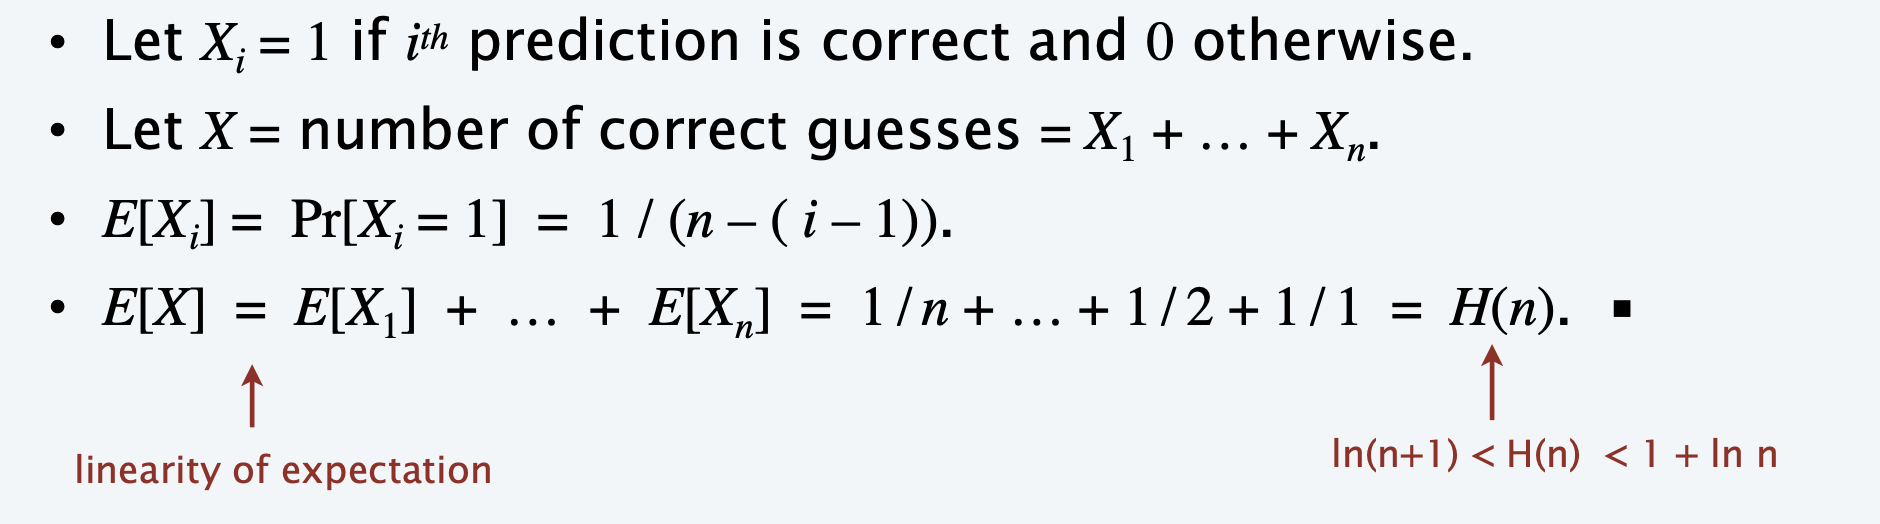
\includegraphics[width=0.6\textwidth ]{card}
\end{figure}

\emph{Coupon Collector}:\\
Each box of cereal contains a coupon, there are n different types of coupons. Assuming all boxes are equally likely to contain each coupon, how many boxes before you have $\geq$ 1 coupon of each type?

\begin{claim}
    The expected number of correct guesses is Θ(nlog n).
\end{claim}\\

\begin{figure}[H]
    \centering
    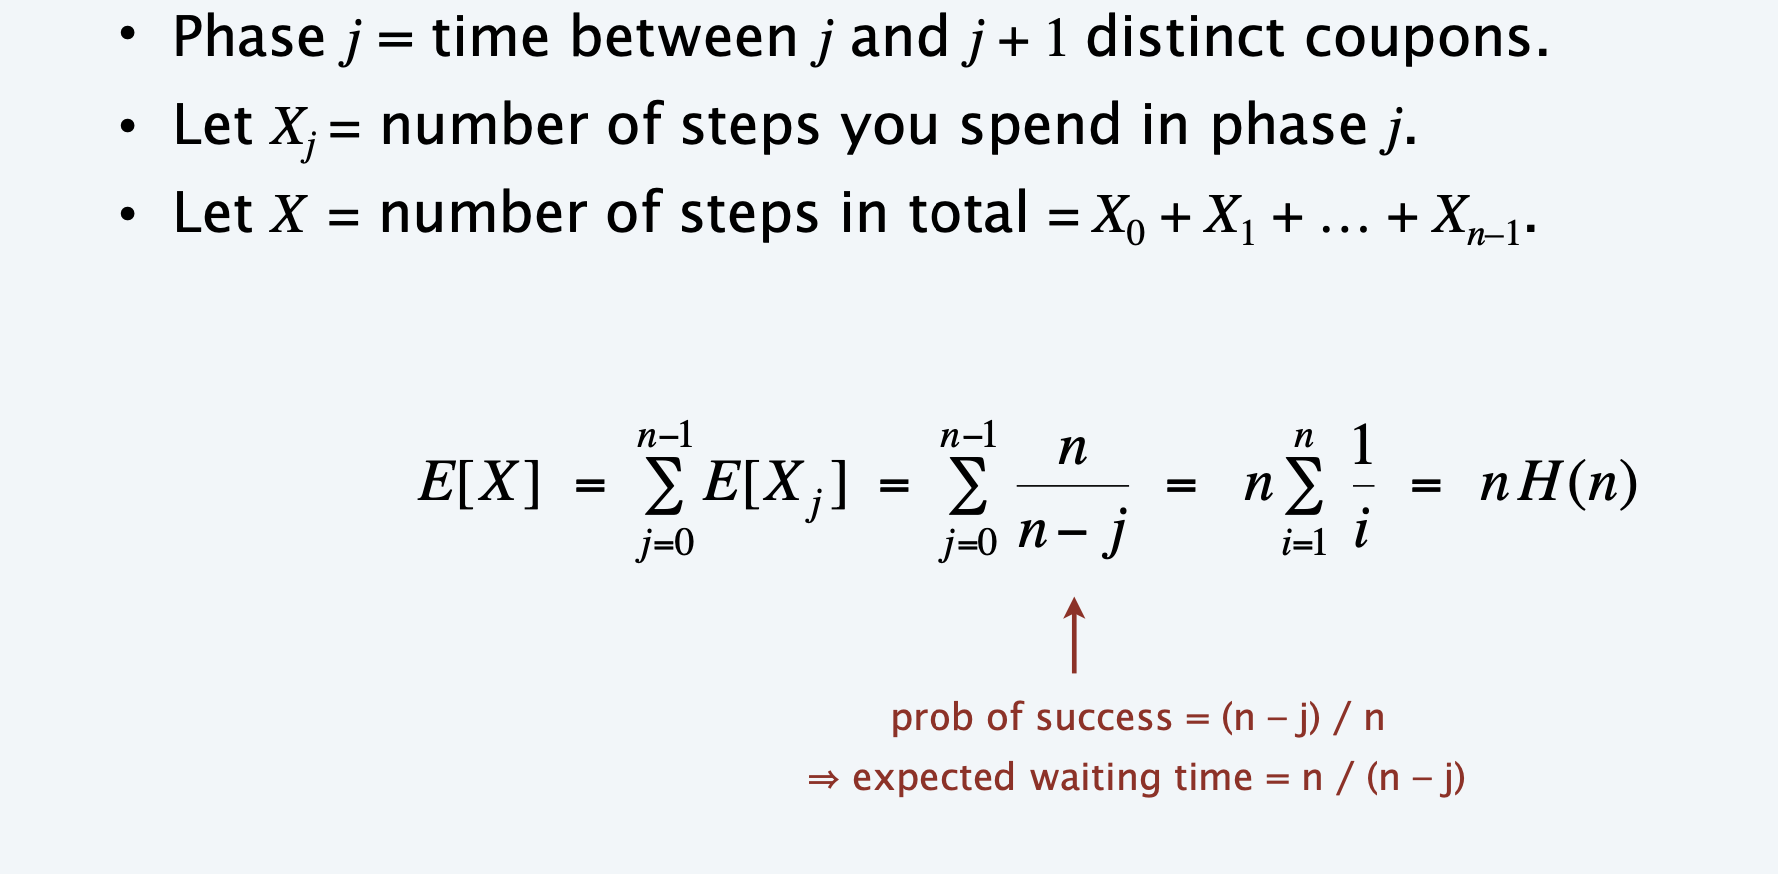
\includegraphics[width=0.6\textwidth ]{coupon}
\end{figure}

\subsection{Monte Carlo vs Las Vegas Algorithms}

\emph{Monte Carlo}: Guaranteed to run in poly-time, likely to find correct answer, ex: contraction algorithm.\\
\emph{Las Vegas}:Guaranteed to find correct answer, likely to run in poly-time.(3-SAT randomized algorithm)\\

It's always possible to convert a Las Vegas algorithm into Monte Carlo,but no known method (in general) to convert the other way.\\

\emph{RP}:Decision problems solvable with one-sided error in poly-time; remark, one side error means: if the correct answer is no, always return no, if it is yes, return yes with probability $\geq \frac{1}{2}$\\\\
\emph{ZPP:}Decision problems solvable in expected poly-time.\\

\[ P \subseteq ZPP \subseteq RP \subseteq NP \]

\subsection{Hashing}

Given a universe U of possible elements, maintain a subset $S \subseteq U$ so that inserting, deleting, and searching in S is efficient, but U can be extremely large so defining an array of size $| U |$ is infeasible.
The hash function is a way to generate a key to immediately identify an element inside a dictionary or encrypt a message:

\[h : U \rightarrow \{ 0, 1, ..., n – 1 \}\]

Create an array a of length n. When processing element u,access array element a[h(u)], a collision occurs when h(u) = h(v) but $u \neq v$ (is expected after Θ(√n)).\\
Obviously it's possible to define deterministic methods for hashing but they are both inefficient ad insecure in real world, our ideal hash function hold the following properties:\\

\begin{itemize}

    \item{Maps m elements uniformly at random to n hash slots.}
    \item{Running time depends on length of chains.}
    \item{Average length of chain = α = $\frac{m}{n}$.}
    \item{Choose n ≈ m ⇒ expect O(1) per insert, lookup, or delete.}

\end{itemize}

The best approach is to use randomization, defining the universal hash function family : $H = \{ h_{a} : a \in A \}$, then:

\[h_{a}(x) = (\sum_{i=1}^{r}a_{i}x_{i}) mod \;p\]

Choose p prime so that $m \leq p \leq 2m$, where m = $| S |$, so we have: Θ(m) space used, the expected number of collisions per operation is $\leq$ 1⇒ O(1) time per insert, delete, or lookup.

\subsection{Marco-Finn Inequality}
The probability of a deviation of the expectation over a factor c is at most $\frac{1}{c}$:
\[ Pr(x>cE[x]) \leq \frac{1}{c}^{c}\]

\subsection{Chernoff Bound}

Random variable that describes the execution of an algorithm, it's equal to the sum of a set of random variables and related to the indipendent sampling of a phenomenon.

\begin{claim}
    Suppose $X_{1}, ..., X_{n}$ are independent 0-1 random variables. Let $X = X_{1} + ... + X_{n}$. Then for any $μ \geq E[X]$ and for any $δ > 0$, we have:

    \[Pr[x>1+δ]μ <[\frac{e^{δ}}{1+δ^{1+δ}}]^{μ }\]
\end{claim}

\begin{claim}
    Suppose $X_{1}, ..., X_{n}$ are independent 0-1 random variables. Let $X = X_{1} + ... + X_{n}$. Then for any $μ \geq E[X]$ and for any $0<δ<1$, we have:

    \[Pr[x>1+δ]μ <e^{-δ^{2}\frac{μ}{2}}\]
\end{claim}


\subsection{Load Balancing}
System in which m jobs arrive in a stream and need to be processed immediately on m identical processors, the jobs are assigned in a  Find an assignment that balances the workload across processors.

\begin{itemize}
    \item{Centralized controller}
          Assign jobs in round-robin manner. Each processor receives at most $\frac{m}{n}$ jobs.
    \item{Decentralized controller}
          Assign jobs to processors uniformly at random. How likely is it that some processor is assigned “too many” jobs?

\end{itemize}

\emph{Notation:}

\begin{itemize}
    \item{$X_{i}$ = number of jobs assigned to processor i.}
    \item{$Y_{ij} = 1$ if job j assigned to processor i, and 0 otherwise.}
\end{itemize}

We have $E[Yij] = \frac{1}{n}$, thus: $Xi = \sum Y_{ij}  ,$ and $μ = E[X_{i}] = 1$.\\\\
Applying the Chernoff bound  with δ = c – 1 yields:

\[ Pr[X_{i} > c] < \frac{e^{c-1}}{c^{c}}\]

\begin{figure}[H]
    \centering
    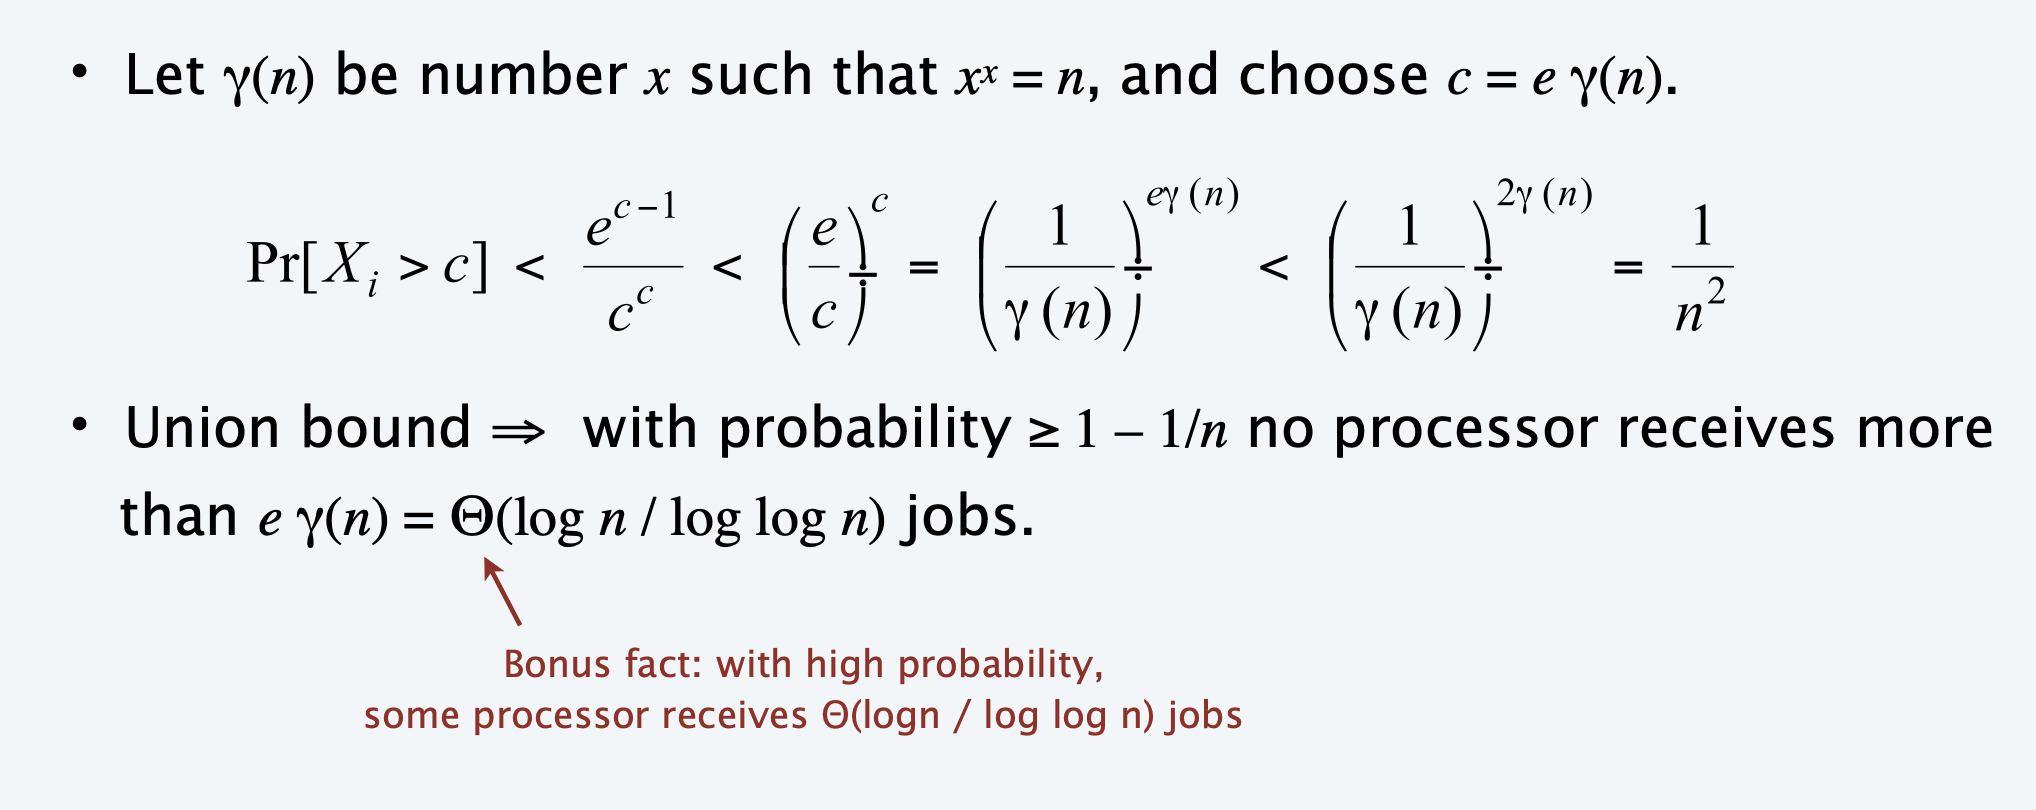
\includegraphics[width=0.6\textwidth ]{job}
\end{figure}

\begin{figure}[H]
    \centering
    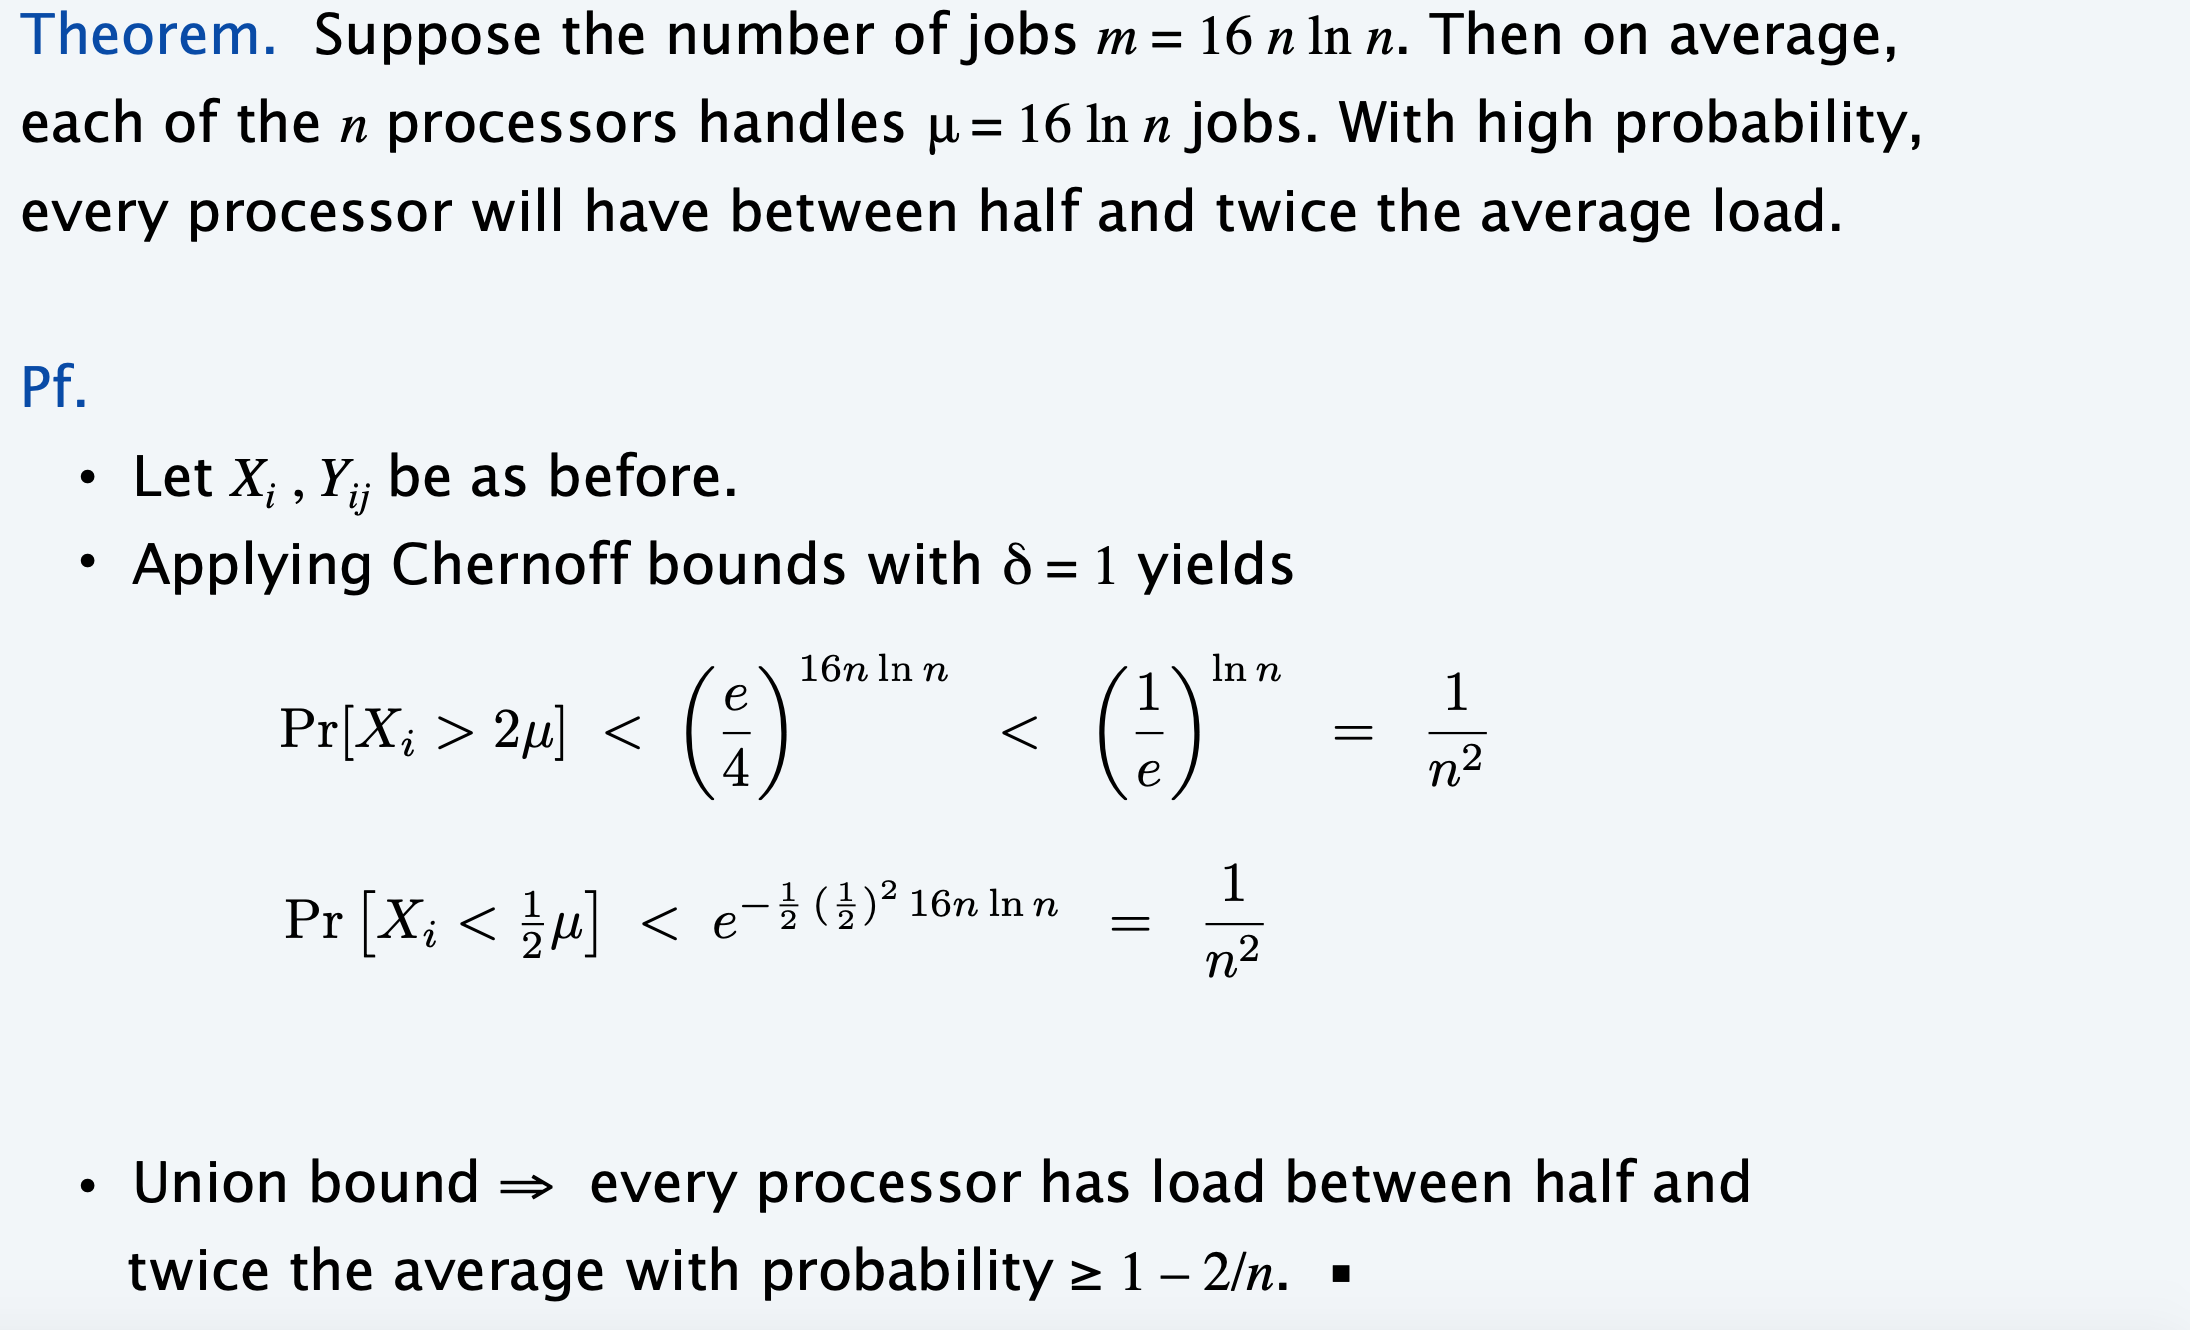
\includegraphics[width=0.6\textwidth ]{jobTh}
\end{figure}

\clearpage
